\documentclass[]{article}
\usepackage{graphicx}

%opening
\title{YJFC Armory App - Equipment Checkout}
\author{Susanna Dong}

\begin{document}

\maketitle

\section{Requirements}
\begin{itemize}
\item JRE 1.8 installed on machine
\end{itemize}

\section{Instructions}
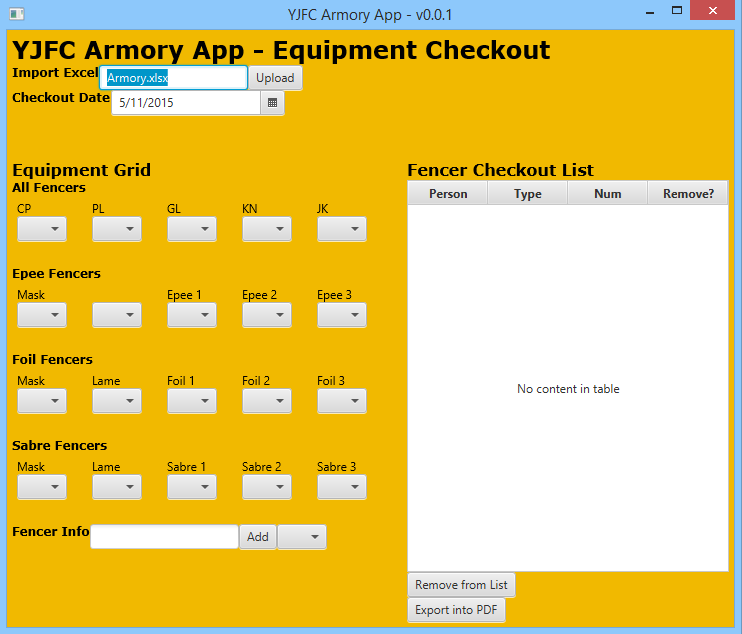
\includegraphics[scale=0.7]{screen.png}

\begin{itemize}
\item \textbf{Import Excel}: Input a valid filepath to an Excel spreadsheet. The Excel spreadsheet format must be .xlsx. Press 'Upload' to upload the spreadsheet into main memory.

\item \textbf{Checkout Date}: Date of checkout. Determines file name of PDF file.

\item \textbf{Equipment Grid}: Grid of equipment filled in with data from Excel spreadsheet.

\item \textbf{Fencer Info}: Two options.
\begin{itemize}
	\item Typing in a fencer's name, selecting the dropdown, and pressing 'Add' will associate all equipment to the fencer.
	\item Clicking the dropdown to the right of the button allows selection of fencer with existing equipment. Clicking 'Deselect' will deselect the existing fencer.
\end{itemize}

\item \textbf{Fencer Checkout List table}: displays all equipment checked out. Clicking the 'Removed' checkbox associated with the equipment and clicking 'Remove from List' will remove the equipment associated with the fencer.

\item \textbf{Export into PDF}: Exports the info displayed in the Fencer Checkout List into a PDF file.
\end{itemize}

\end{document}
